% $Id:experiments.tex  $
% !TEX root = main.tex

\chapter{experiments}
\label{cha:experiments}
Many options were taken in count while selecting environment to apply the transfer learning technique. The first one was CARLA \cite{CARLA}, which provides a realistic and dynamic context for autonomous driving research. In the frame of the MDP a reward signal was chosen to incentivize the agent to maintain a target speed of 50 km/h. The simulation environment for this study is the CARLA urban driving simulator.

Given that this document is employing a Twin Delayed Deep Deterministic Policy Gradient for decision-making, the action space has three continuous signals that can be powered: steering the vehicle, Throttle the vehicle, or break, CARLA simulator provides a way to manually shift gears and press the hand break, however in this experiment the car is only going to be able to move forward and the the gear shifting is going to be automatic. The vehicle is going to have one sensor only which is going to be an rgb frontal camera attached to the roof of the vehicle which is going to produce images of 3 rgb channels of 480 x 640 pixels. The reward function is designed to encourage the agent to reach and sustain the desired speed of $50km/h$ while navigating through the environment. This approach ensures that the agent learns to balance the need for speed with the challenges of urban driving, such as handling turns and avoiding obstacles. To achieve this, the agent receives a penalty of $-1$ for every step taken that is not above the $50km/h$, and gets a penalty of $-200$ for a collision and a negative reward of $-15$ every time it changes lane in a forbidden area.

\begin{figure}[!ht]
    \centering

    \subfloat[][Carla catalogue Townt 5 Overview.]{
        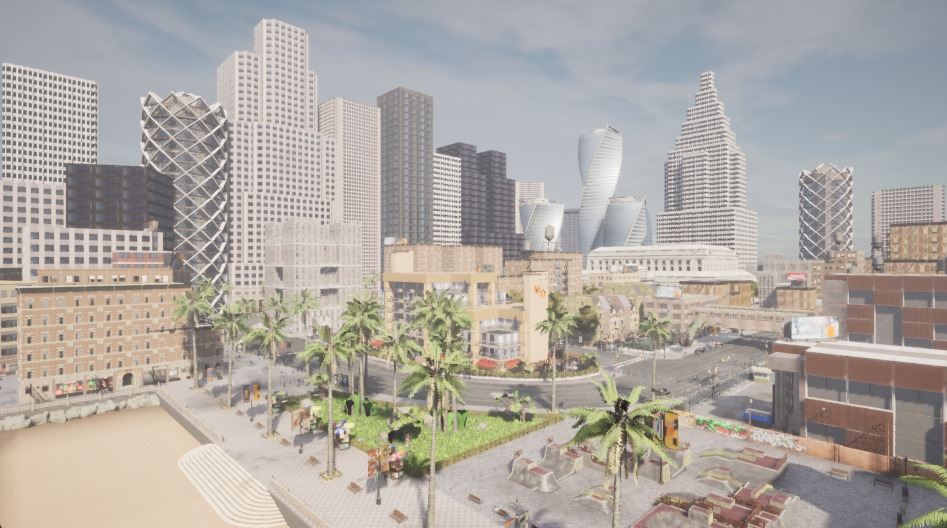
\includegraphics[width=0.98\textwidth]{figures/town5_carla_view1.png}
    }

    \subfloat[][Carla catalogue Townt 5 Overview.]{
        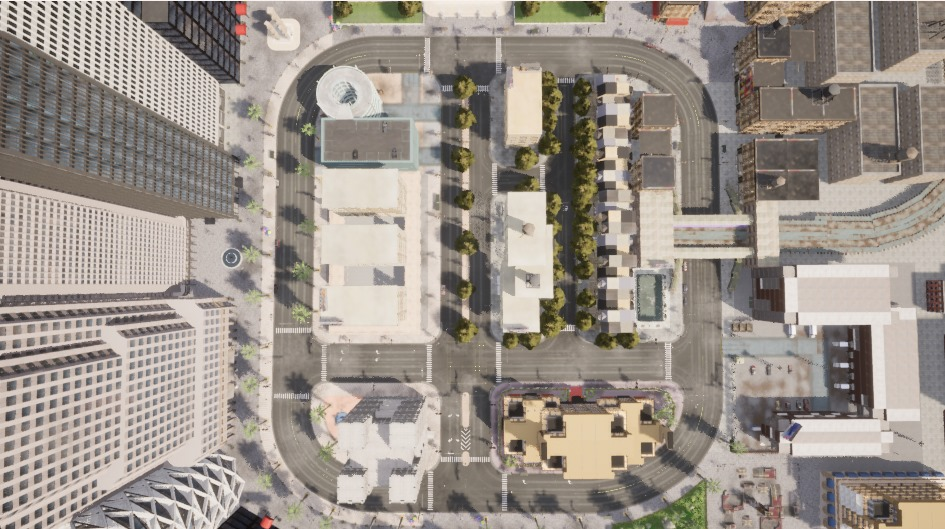
\includegraphics[width=0.98\textwidth]{figures/town5_carla_top_view.png}
    }

    \caption{Town 5 of Carla catalogue.}
    \label{fig:town 5 carla}
\end{figure}

\cite[Xception]{XCeption} is a 71 layer deep convolutional neural network which has over 23 millions trainable parameters. It was utilized to act as a policy function of the DDPG algorithm, for the critic network, a 4 layered of convolutional model followed by 2 dense layers was used to predict the value function of the actor in the environment.

The agent in the simulator was chosen to be a Cybertruck, model provided by the simulator as shown in figure \ref{cybwertruck carla}. CARLA provides in its catalogue a list of maps for use. For the experiment it was used the \ref{fig:town 5 carla} is an urban area nestled against conifer-covered hills, featuring a raised highway and expansive multilane roads with several major intersections.

\begin{figure}[ht]
    \centering
    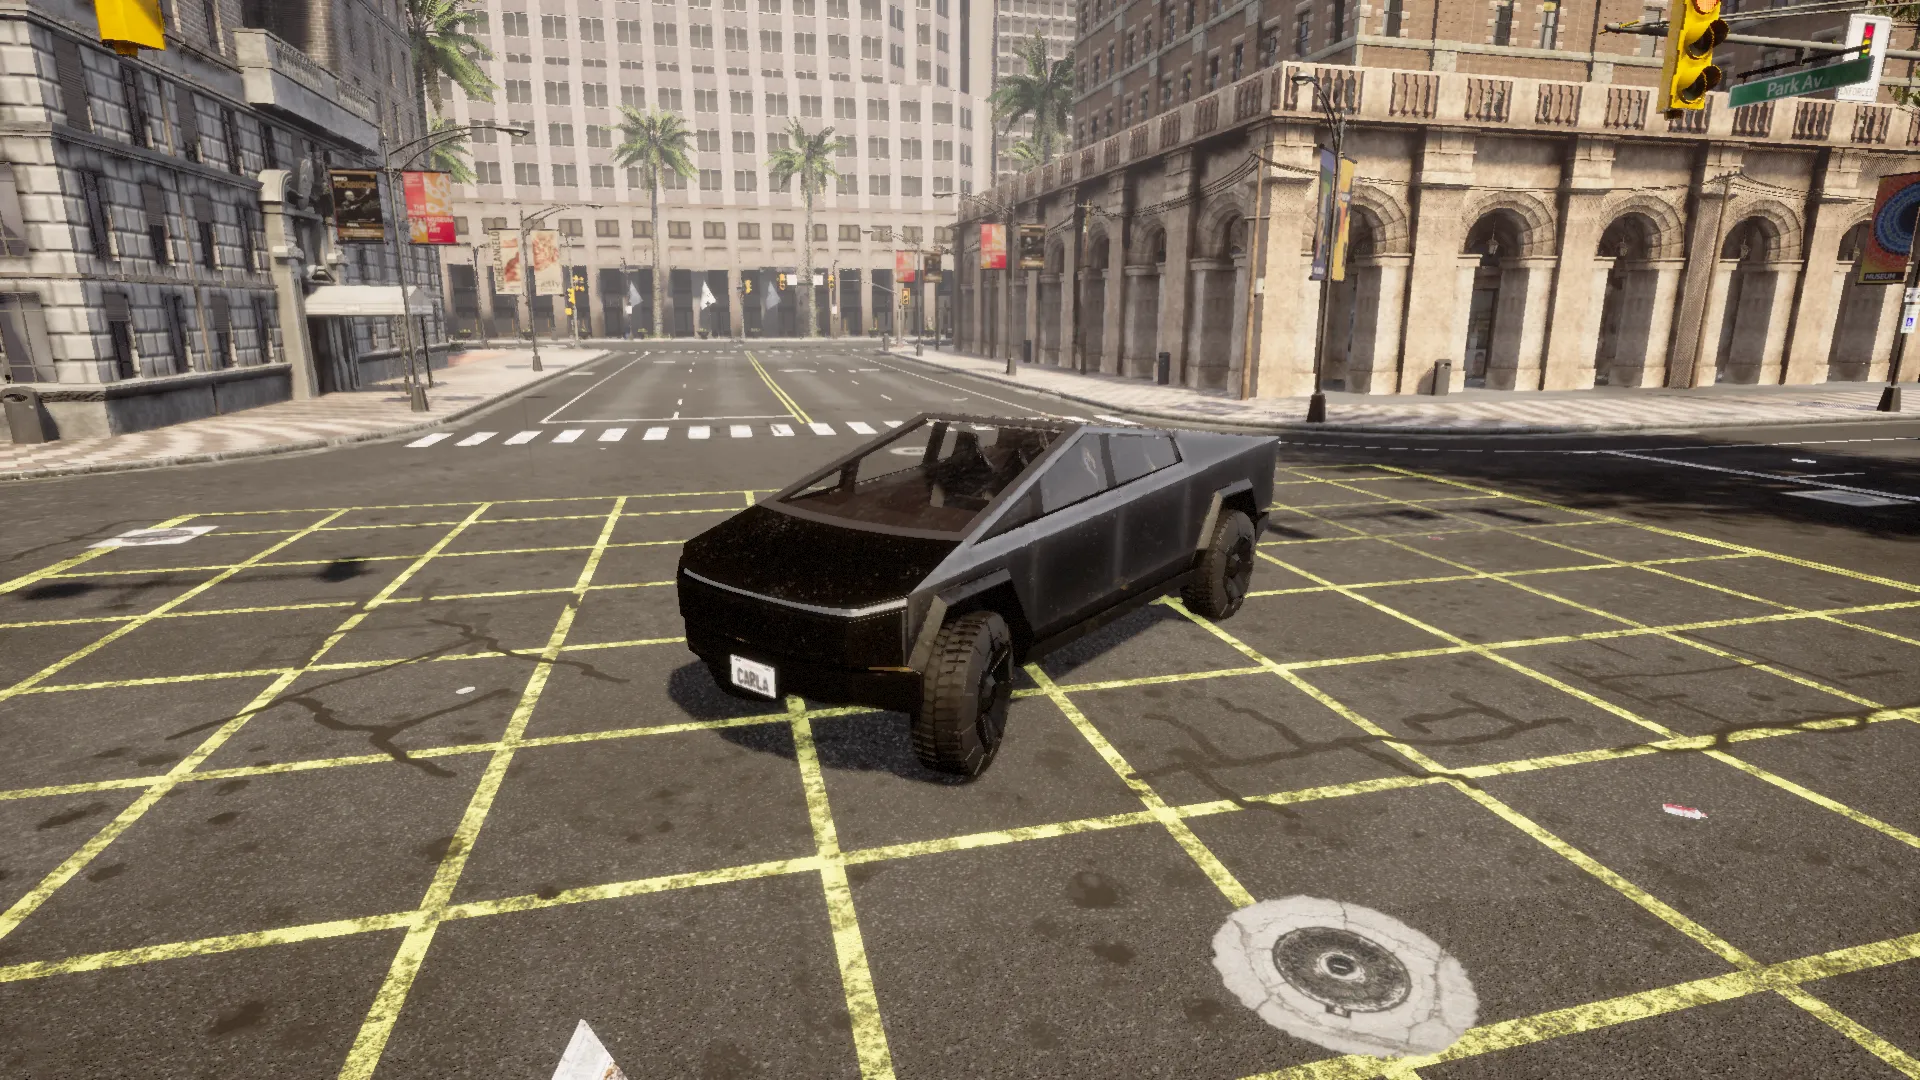
\includegraphics[width=1.0\textwidth]{./figures/tesla_cybertruck_carla.png}
    \caption{Cybertruck model in Carla environment in Town 5.}
    \label{cybwertruck carla}
\end{figure}

With this experiment it was possible to train up to 32.000 iterations, however, due to technical difficulties related with the hardware, and the model being computationally expensive, it was not possible to train any further. and even though as shown in figure the reward seems to go up, the variance through episodes is high. From this point, it was decided to change the simulator and hence the environment.

\begin{figure}[ht]
    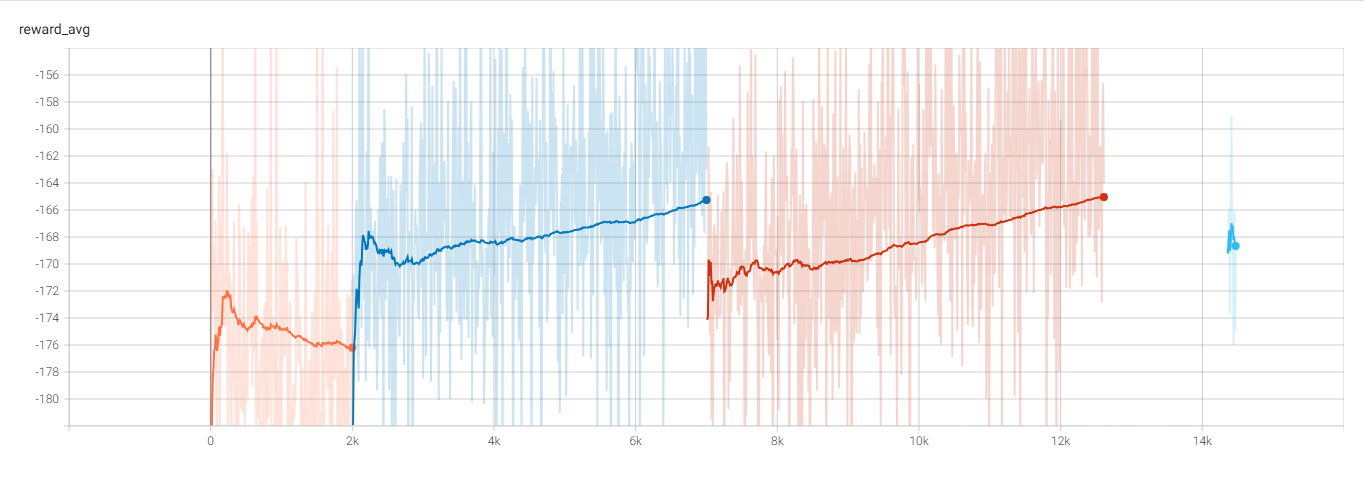
\includegraphics[width=1.0\textwidth]{./figures/CARLA_ddpg_14k_iters.png}
    \caption{CARLA DDPG Cybertruck train log, 14000 iterations.}
\end{figure}

The next experiment was performed in Gazebo simulator and the Turtlebot3 mobile base shown in figure \ref{fig: tb3 model burger}, a differential mobile base with a Lidar\footnote{Laser Distance Sensor: https://emanual.robotis.com/docs/en/platform/turtlebot3/appendix\_lds\_01/}. It was tried on different network architectures for the training with the same set of hyperparameters settings across all the the models, it was chosen a model composed of 3 Dense\footnote{A dense layer is a simple Layer of neurons in which each neuron receives input from all the neurons of the previous layer: \url{https://keras.io/api/layers/core\_layers/dense}.} layers, the input of the network is the measurement received from the Lidar sensor which consist of 26 measurement of detected distances in angles around the mobile base plus the $x$ and $y$ distance of the goal from the mobile base. The reward functions was designed to encourage the mobile base to get from its start point to the goal point in the less episodes possible and discouraging crash against any obstacle and keeping only on one side of the road. A crash of any kind is catastrophic for the episode.

\begin{figure}[ht]
    \centering
    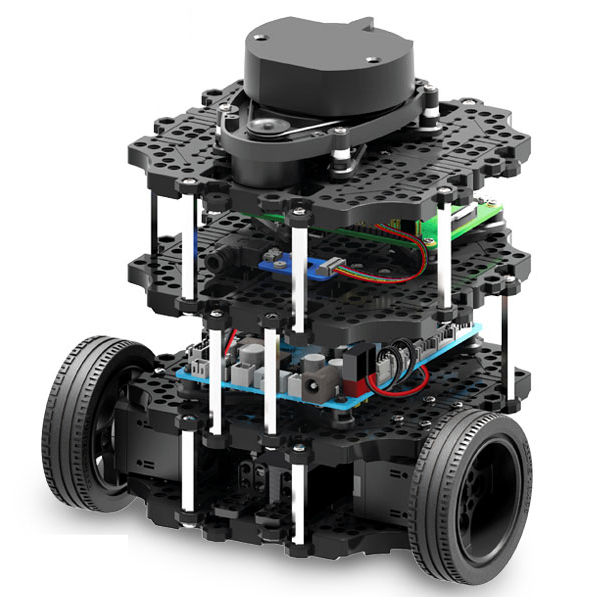
\includegraphics[width=0.2\textwidth]{./figures/turtlebor3_burger.png}
    \caption{Turtlebot3 model Burger.}
    \label{fig: tb3 model burger}
\end{figure}

To emulate the driving paradigm change, it was built an environment of a roundabout with line tracks emulated by walls as shown in figure \ref{fig: gazebo tb3 environment}. The blue layer represent what the robot "sees" through the Lidar scans. For each episode the robot is going to start from one side of the environment and should learn to go to the other side of the environment following only one track of the road, then, another agent is going to be trained with a brand new actor and critic models to follow the other track of the road so at the end there are two agents, one that knows how to traverse the environment following the right side and the other ones knows the other paradigm.

\begin{figure}[ht]
    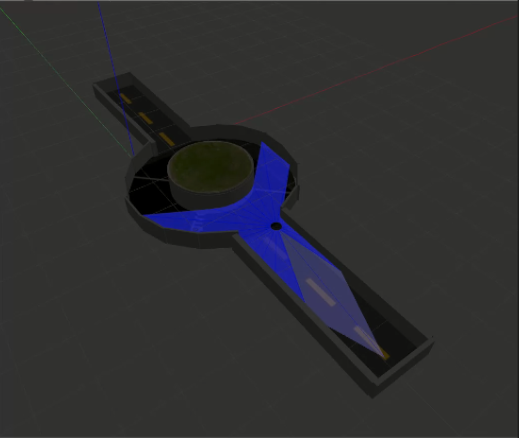
\includegraphics[width=0.7\textwidth]{./figures/experiment_environment_gazebo.png}
    \centering
    \caption{Turtlebot 3 in Gazebo simulator with roundabout environment.}
    \label{fig: gazebo tb3 environment}
\end{figure}

Once the two agents are trained, the main idea is to transfer the knowledge from one agent to the other via transfer learning, and measuring the transferred knowledge by 3 metrics given by the following equations:

\begin{equation}
    \begin{split}
        \text{Transfer ratio} & = \frac{\text{Ultimate performance with TL}}{\text{Ultimate performance with no TL}} \\
        Mastery               & = \text{Ultimate performance of the} agent.                                          \\
        Pedagogy              & = \text{How many less episodes the TL agent takes than a 0 trained agent.}
    \end{split}
\end{equation}

Where the $Ultimate performance$ means the return of the episode or the discounted cumulative reward achieved by the agent at the end of the episode.